% Plane Sections of the Cylinder - Dandelin Spheres
% Author: Hugues Vermeiren
\documentclass{article}
\usepackage{tikz}
\tikzset{
	MyPersp/.style={scale=1.8,x={(-0.8cm,-0.4cm)},y={(0.8cm,-0.4cm)},
    z={(0cm,1cm)}},
%  MyPersp/.style={scale=1.5,x={(0cm,0cm)},y={(1cm,0cm)},
%    z={(0cm,1cm)}}, % uncomment the two lines to get a lateral view
	MyPoints/.style={fill=white,draw=black,thick}
		}
\begin{document}

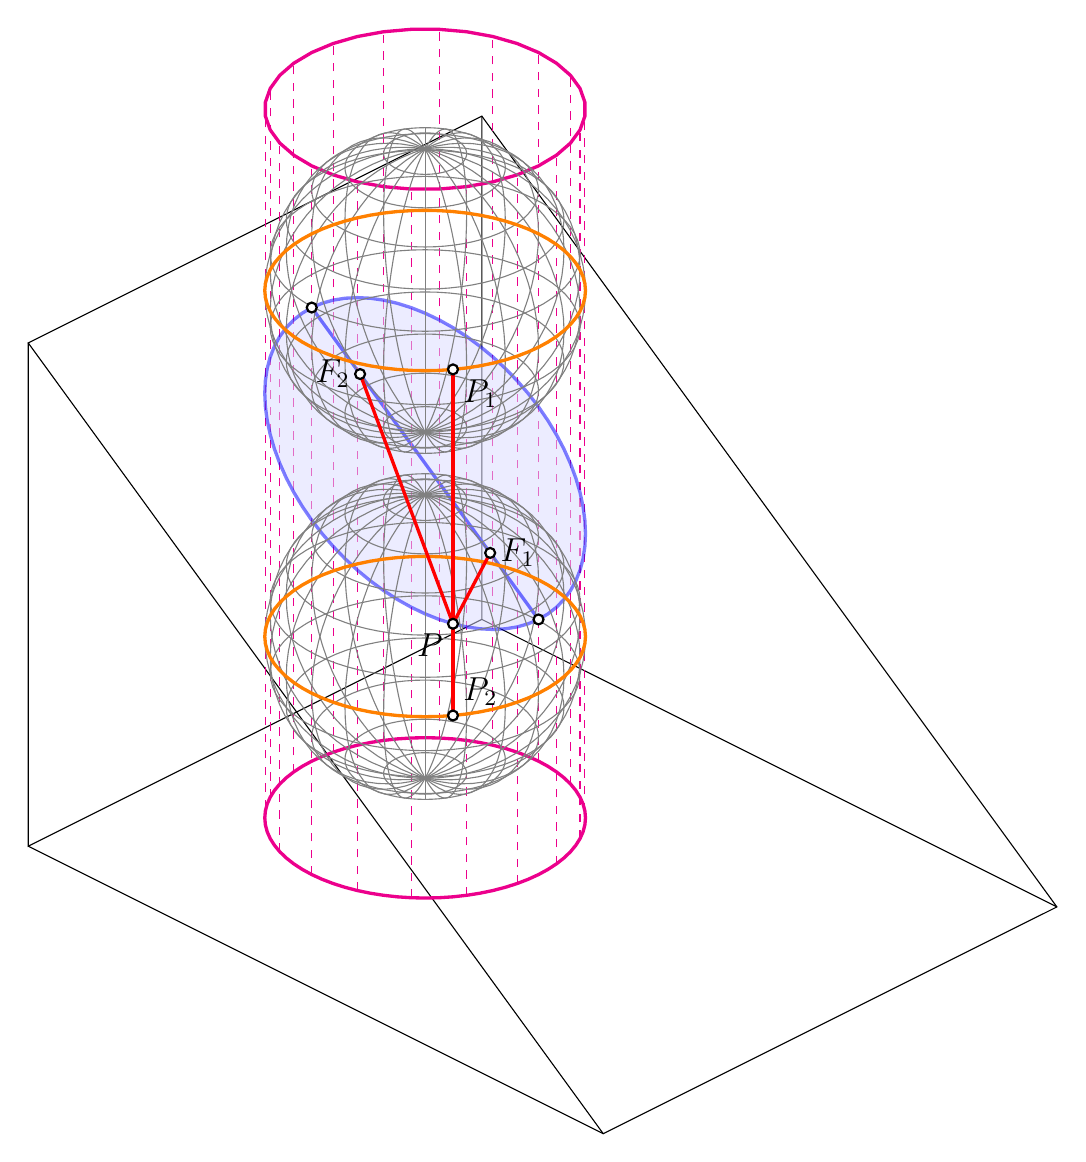
\begin{tikzpicture}[MyPersp,font=\large]
	% the base circle is the unit circle in plane Oxy
	\def\h{2.5}% Heigth of the ellipse center (on the axis of the cylinder)
	\def\a{35}% angle of the section plane with the horizontal
	\def\aa{35}% angle that defines position of generatrix PA--PB
	\pgfmathparse{\h/tan(\a)}
  \let\b\pgfmathresult
	\pgfmathparse{sqrt(1/cos(\a)/cos(\a)-1)}
  \let\c\pgfmathresult %Center Focus distance of the section ellipse.
	\pgfmathparse{\c/sin(\a)}
  \let\p\pgfmathresult % Position of Dandelin spheres centers
                       % on the Oz axis (\h +/- \p)
	\coordinate (A) at (2,\b,0);
	\coordinate (B) at (-2,\b,0);
	\coordinate (C) at (-2,-1.5,{(1.5+\b)*tan(\a)});
	\coordinate (D) at (2,-1.5,{(1.5+\b)*tan(\a)});
	\coordinate (E) at (2,-1.5,0);
	\coordinate (F) at (-2,-1.5,0);
	\coordinate (CLS) at (0,0,{\h-\p});
	\coordinate (CUS) at (0,0,{\h+\p});
	\coordinate (FA) at (0,{\c*cos(\a)},{-\c*sin(\a)+\h});% Focii
	\coordinate (FB) at (0,{-\c*cos(\a)},{\c*sin(\a)+\h});
	\coordinate (SA) at (0,1,{-tan(\a)+\h}); % Vertices of the
                                           % great axes of the ellipse
	\coordinate (SB) at (0,-1,{tan(\a)+\h});
	\coordinate (PA) at ({sin(\aa},{cos(\aa)},{\h+\p});
	\coordinate (PB) at ({sin(\aa},{cos(\aa)},{\h-\p});
	\coordinate (P) at ({sin(\aa)},{cos(\aa)},{-tan(\a)*cos(\aa)+\h});
     % Point on the ellipse on generatrix PA--PB

	\draw (A)--(B)--(C)--(D)--cycle;
	\draw (D)--(E)--(F)--(C);
	\draw (A)--(E) (B)--(F);
	\draw[blue,very thick] (SA)--(SB);

%	\coordinate (O) at (0,0,0);
%	\draw[->] (O)--(2.5,0,0)node[below left]{x};
%	\draw[->] (O)--(0,3,0)node[right]{y};
%	\draw[->] (O)--(0,0,6)node[left]{z};

	\foreach \t in {20,40,...,360}% generatrices
		\draw[magenta,dashed] ({cos(\t)},{sin(\t)},0)
      --({cos(\t)},{sin(\t)},{2.0*\h});
	\draw[magenta,very thick] (1,0,0) % lower circle
		\foreach \t in {5,10,...,360}
			{--({cos(\t)},{sin(\t)},0)}--cycle;
	\draw[magenta,very thick] (1,0,{2*\h}) % upper circle
		\foreach \t in {10,20,...,360}
			{--({cos(\t)},{sin(\t)},{2*\h})}--cycle;
	\fill[blue!15,draw=blue,very thick,opacity=0.5]
     (0,1,{\h-tan(\a)}) % elliptical section
		\foreach \t in {5,10,...,360}
			{--({sin(\t)},{cos(\t)},{-tan(\a)*cos(\t)+\h})}--cycle;

	\foreach \i in {-1,1}{%Spheres!
		\foreach \t in {0,15,...,165}% meridians
			{\draw[gray] ({cos(\t)},{sin(\t)},\h+\i*\p)
				\foreach \rho in {5,10,...,360}
					{--({cos(\t)*cos(\rho)},{sin(\t)*cos(\rho)},
          {sin(\rho)+\h+\i*\p})}--cycle;
			}
		\foreach \t in {-75,-60,...,75}% parallels
			{\draw[gray] ({cos(\t)},0,{sin(\t)+\h+\i*\p})
				\foreach \rho in {5,10,...,360}
					{--({cos(\t)*cos(\rho)},{cos(\t)*sin(\rho)},
          {sin(\t)+\h+\i*\p})}--cycle;
			}
					\draw[orange,very thick] (1,0,{\h+\i*\p})% Equators
		\foreach \t in {5,10,...,360}
			{--({cos(\t)},{sin(\t)},{\h+\i*\p})}--cycle;
		}
	\draw[red,very thick] (PA)--(PB);
	\draw[red,very thick] (FA)--(P)--(FB);
%	\fill[MyPoints] (CLS) circle (1pt);% center of lower sphere
%	\fill[MyPoints] (CUS) circle (1pt);% center of upper sphere
	\fill[MyPoints] (FA) circle (1pt)node[right]{$F_1$};
	\fill[MyPoints] (FB) circle (1pt)node[left]{$F_2$};
	\fill[MyPoints] (SA) circle (1pt);
	\fill[MyPoints] (SB) circle (1pt);
	\fill[MyPoints] (P) circle (1pt)node[below left]{$P$};
	\fill[MyPoints] (PA) circle (1pt)node[below right]{$P_1$};
	\fill[MyPoints] (PB) circle (1pt)node[above right]{$P_2$};
\end{tikzpicture}

\end{document}